\documentclass[aspectratio=169]{beamer}
\usepackage{listings}
\usepackage[utf8]{inputenc}
\usepackage[T1]{fontenc}
\usepackage{subfigure}
\usepackage{xcolor}
\usepackage{tikz}
\usepackage{tikzscale}
\usetikzlibrary{decorations.pathreplacing}
\usetikzlibrary{calc}
\usetikzlibrary{shapes,snakes}
\usetikzlibrary{patterns}
% BIBLIOGRAPHY
\usepackage[style=numeric, 
            backend=biber,
            giveninits=true]{biblatex}
\setbeamertemplate{bibliography item}{\insertbiblabel}
\addbibresource{bibliography.bib}
% MATH
\usepackage{amsmath,amsfonts,amssymb,amsthm} % For math equations, theorems, symbols, etc
\usepackage{mathtools}
\usepackage{dsfont}



%
% TIKZ equation terms' highlight
%% https://tex.stackexchange.com/questions/458694/highlighting-part-of-equation-with-text-underneath
\usetikzlibrary{tikzmark}
\tikzset{upper node/.style={inner sep=2,fill=blue!10},
lower node/.style={inner sep=1,ellipse,fill=blue!3},
ul line/.style={thick,blue!20},
upper/.code={\tikzset{upper node/.append style={#1}}},
lower/.code={\tikzset{lower node/.append style={#1}}},
line/.code={\tikzset{ul line/.append style={#1}}},
}
\newcounter{HighLight}
\newcommand{\highlight}[3][]{%
\stepcounter{HighLight}
\tikzset{#1}
\underset{\underset{\displaystyle\makebox[0pt]{\text{\tikzmarknode[lower node]{below-\theHighLight}{%
#3}}}}{\phantom{!}}}{\tikzmarknode[upper node]{above-\theHighLight}{#2}}
\tikz[overlay,remember picture]{\draw[ul line] (above-\theHighLight) --
(below-\theHighLight);}
}




\definecolor{codegreen}{rgb}{0,0.6,0}
\definecolor{codegray}{rgb}{0.5,0.5,0.5}
\definecolor{codepurple}{rgb}{0.58,0,0.82}
\definecolor{backcolour}{rgb}{0.95,0.95,0.92}
\lstdefinestyle{mystyle}{
    backgroundcolor=\color{backcolour},
    commentstyle=\color{codegreen},
    keywordstyle=\color{magenta},
    numberstyle=\tiny\color{codegray},
    stringstyle=\color{codepurple},
    basicstyle=\ttfamily\footnotesize,
    breakatwhitespace=false,
    breaklines=true,
    captionpos=b,
    keepspaces=true,
    numbers=left,
    numbersep=5pt,
    showspaces=false,
    showstringspaces=false,
    showtabs=false,
    tabsize=2
}
\lstset{style=mystyle}


\title{NFV Orchestration in Edge and Fog Scenarios}
\date{26\textsuperscript{th} October, 2021}
\author{
    {\footnotesize \textit{student}}: \! \! \! J. Martín-Pérez\\
    {\footnotesize \textit{supervisor}}: C. J. Bernardos\\
    \vspace{2em}
    \footnotesize{\textit{contact}: \href{mailto:jmartinp@it.uc3m.es}{jmartinp@it.uc3m.es}}
}

\usetheme{uc3m}

\begin{document}

\begin{frame}
\titlepage
\end{frame}

\setcounter{framenumber}{0}


\begin{frame}
    \frametitle{Outline}
    \tableofcontents[hideallsubsections,pausesections]
\end{frame}



\section{Generation of 5G infrastructure graphs}
\subsection{State of the art}
\begin{frame}
    \frametitle{Outline}
    \tableofcontents[subsectionstyle=show/shaded/hide,sectionstyle=show/shaded]
\end{frame}

\begin{frame}
    \frametitle{\secname}
    \framesubtitle{\subsecname}
    %
    \textbf{Location of BSs}:
    \begin{itemize}
        \item Neyman-Scott Poisson Cluster Process~\cite{vinay-moller-interference}
        \item Poisson Point Processes (PPPs)~\cite{stochastic-martina}
            \begin{itemize}
                \item homogeneous~\cite{cran-vinay-moller,hetnets-cor}
                \item hard-core~\cite{hard-core-cover} \pause
                \item {\color{red}\textbf{inhomogeneous \& Matérn~II}}
            \end{itemize}
    \end{itemize}
    \pause
    \vfill
    \hrule
    \vfill
    \textbf{Location of MEC PoPs}:
    \begin{itemize}
        \item along highways~\cite{usa-mec}
        \item within stadiums~\cite{tokio-olympics} \pause
        \item {\color{red}\textbf{population census}}
        \item {\color{red}\textbf{access \& aggregation rings}}
    \end{itemize}

\end{frame}


\subsection{Thesis contributions}
\begin{frame}
    \frametitle{Outline}
    \tableofcontents[subsectionstyle=show/shaded/hide,sectionstyle=show/shaded]
\end{frame}



\begin{frame}
    \frametitle{\secname}
    \framesubtitle{\subsecname}
    \vfill
    \begin{minipage}{0.27\textwidth}
        Derive:
        \begin{itemize}
            \item BS location
            \item MEC PoP location
        \end{itemize}
        Meet:
        \begin{itemize}
            \item Tactile RTT of \mbox{\textbf{1 ms}}
        \end{itemize}
    \end{minipage}
    \hfill
    \begin{minipage}{0.68\textwidth}
        \begin{figure}
            \centering
            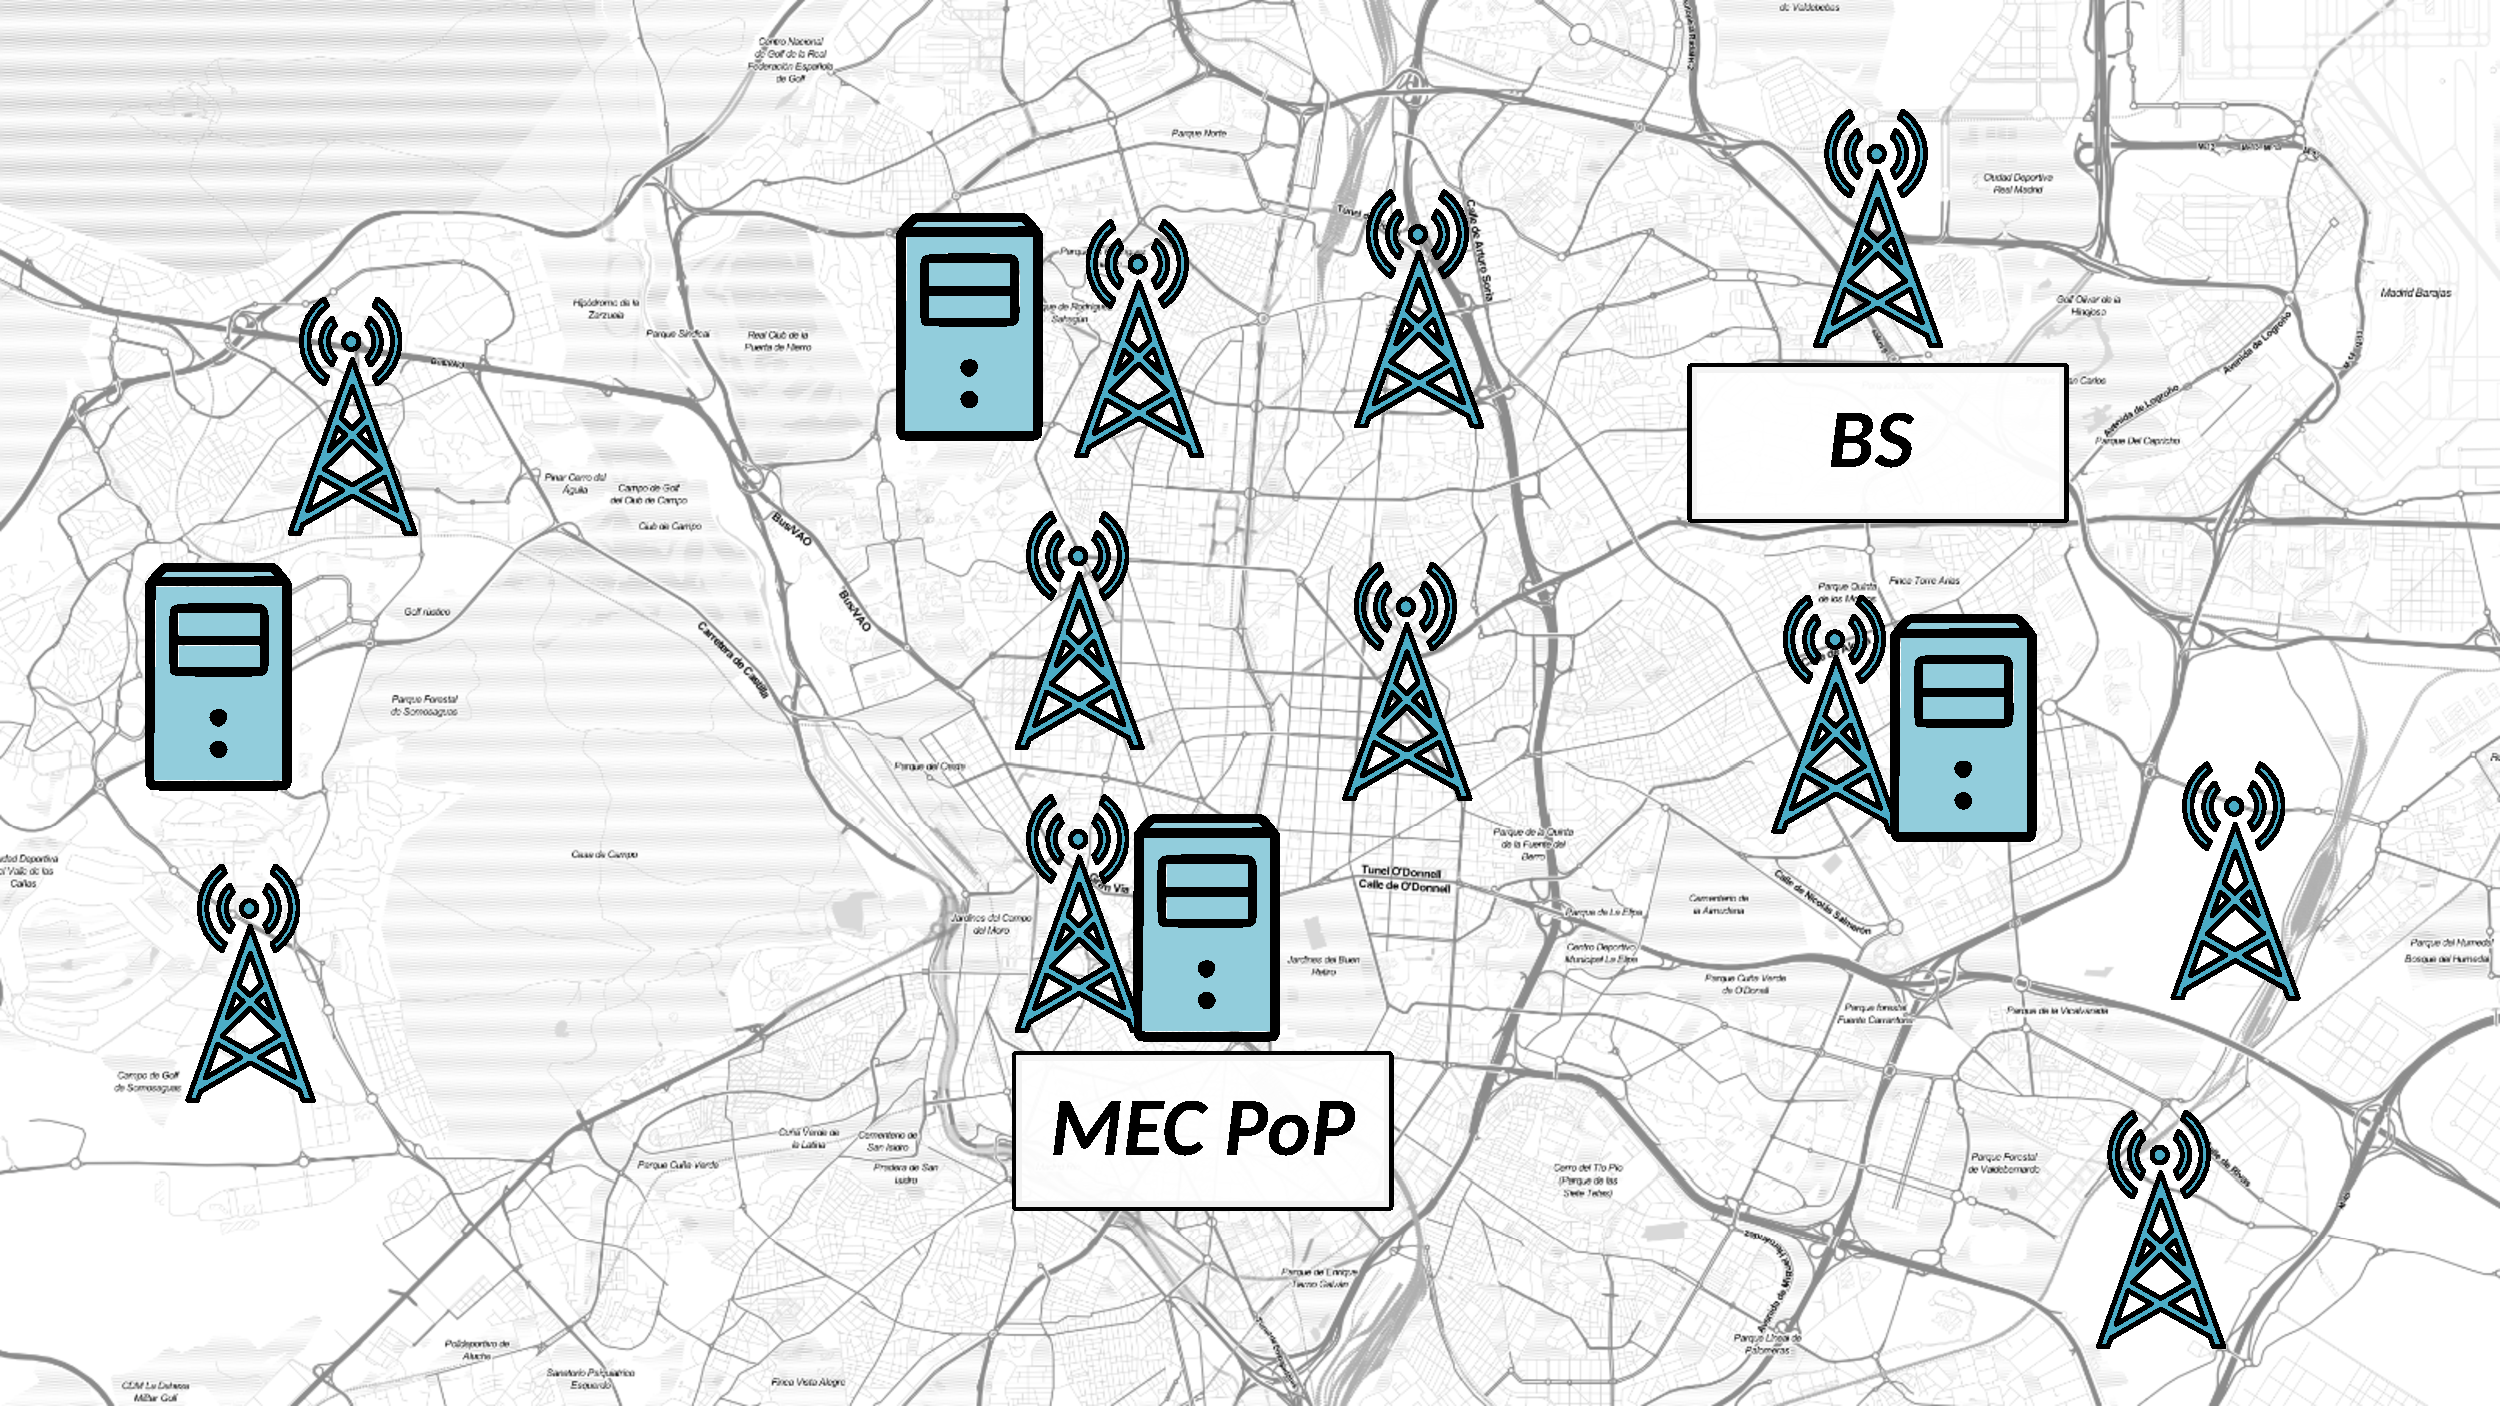
\includegraphics[width=\textwidth]{img/pop-and-antennas.pdf}
            \caption{BS and MEC PoP locations}
            \label{fig:bs-pop-locations}
        \end{figure}
    \end{minipage}
    \vfill
\end{frame}




\begin{frame}
    \frametitle{\secname}
    \framesubtitle{\subsecname}

    Higher gentrification $\implies$ more BSs
    \vfill

    \begin{minipage}{.35\textwidth}
        \begin{itemize}
            \item $f_i(x)$ -- revolution func.
            \item $G(x)$ -- gentrification
            \item $R$ -- region of interest
            \item $C_i$ -- area
        \end{itemize}
    \end{minipage}
    \begin{minipage}{.64\textwidth}
        \begin{figure}
            \centering
            \begin{tikzpicture}
                \node[inner sep=0pt] (russell) at (0,0) {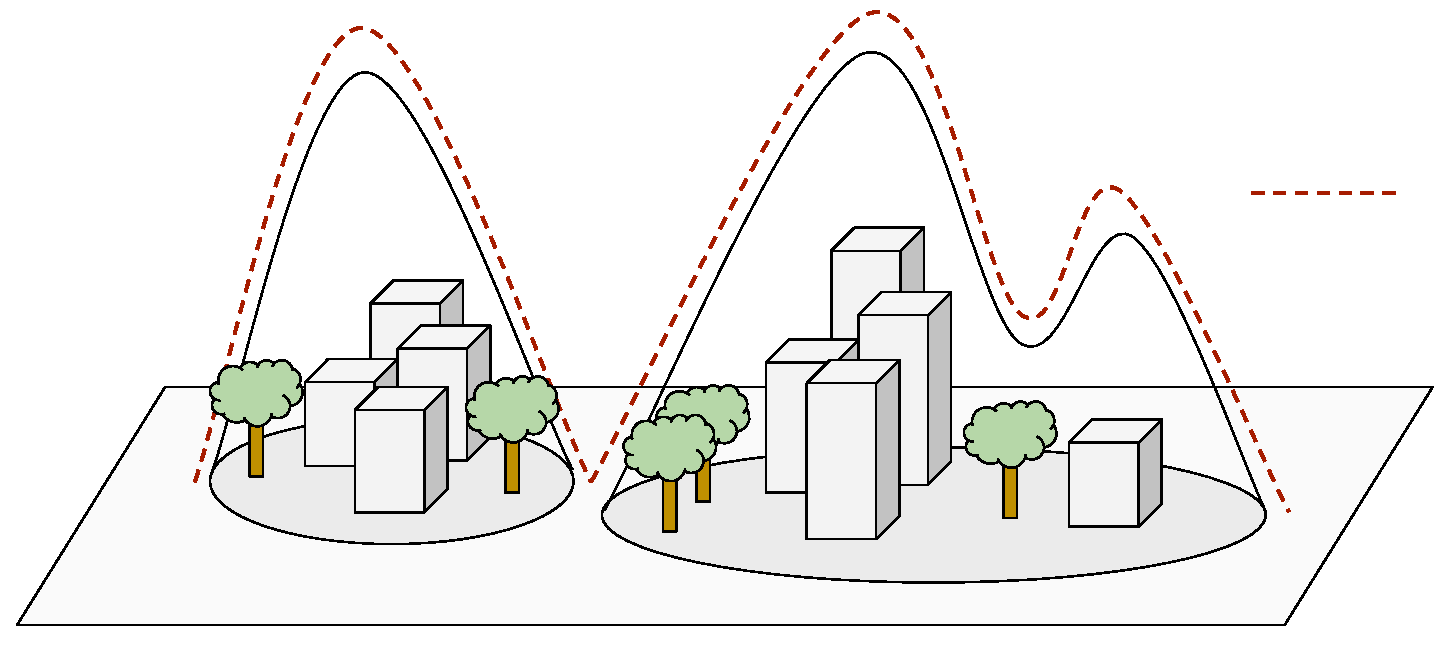
\includegraphics[width=\textwidth]{img/revolution-function}};
                \node at (-2.2,1) {$f_1$};
                \node at (.9,1.2) {$f_2$};
                \node at (-2.6,-1.5) {$C_1$};
                \node at (-.4,-1.6) {$C_2$};
                \node at (3.6, 1.2) {$G(x)$};
                \node at (-4,-1.65) {$R$};
            \end{tikzpicture}
            \caption{\emph{Revolution functions} of a region with two building areas.}
            \label{fig:rev}
        \end{figure}
    \end{minipage}

\end{frame}





\begin{frame}
    \frametitle{\secname}
    \framesubtitle{\subsecname}

    BS intensity function $\lambda(x)\sim G(x)$ proportional to gentrification.

    \vfill

    \begin{figure}
        \centering
        \begin{tikzpicture}[scale=.65,every node/.style={scale=0.65}]
    %%%%%%%%%%%%%%%%%%%%%
    % Gridded rectangle %
    %%%%%%%%%%%%%%%%%%%%%
    % Top brace
    \draw [ultra thick, decorate,decoration={brace,amplitude=4pt}] (2.2,5.2) -- (3.3,5.2) node [black,midway,yshift=0.5cm] {};

    \draw (0,0) rectangle (5,5);
    \foreach \c in {1.1, 2.2, 3.3, 4.4} {
        \draw[dashed, color=gray] (\c, 0) -- (\c, 5);
    }
    \foreach \r in {3.9, 2.8, 1.7, 0.6} {
        \draw[dashed, color=gray] (0, \r) -- (5, \r);
    }


    % Area names
    \edef\index{0}
    \foreach \r in {5, 3.9, 2.8, 1.7, 0.6} {
        \foreach \c in {0, 1.1, 2.2, 3.3, 4.4} {
            \node at (\c + 0.3, \r - 0.25) {\small{$R_{\index}$}};
            \pgfmathparse{int(\index+1)}
            \xdef\index{\pgfmathresult}
        }
    }

    % hashed area
    \draw[fill=white] (2.2,5) rectangle (3.3,3.9);
    \draw[pattern=north west lines, pattern color=black] (2.2,5) rectangle (3.3,3.9);
    \draw[fill=white] (2.27, 4.95) rectangle (2.7, 4.6);
    \node[name=highlighted] at (2.5, 4.75){\small{$R_2$}};

    % Top left coordinate
    \draw[fill=black] (0,5) circle [radius=2.5pt];
    \node at (0, 5.4) {$(x_{1,l},\ x_{2,t})$};

    % Bottom right coordinate
    \draw[fill=black] (5,0) circle [radius=2.5pt];
    \node at (5, -0.4) {$(x_{1,r},\ x_{2,b})$};

    % x1 side
    \draw[|-|] (1.1, -0.2) -- (2.2, -0.2);
    \node at (1.6, -0.5) {$x_{1,s}$};

    % x2 side
    \draw[|-|] (-0.2, 0.6) -- (-0.2, 1.6);
    \node at (-0.6, 1.1) {$x_{2,s}$};

    % Region tag
    \node at (2.5, -1) {\large{$R$}};


    %%%%%%%%%%%%%%%%%%
    % AAUs Matern II %
    %%%%%%%%%%%%%%%%%%
    \draw (2.75,5.3) -- (2.75, 5.65) -- (9.5, 5.65) -- (9.5, 5.5);
    % Top brace
    \draw [ultra thick, decorate,decoration={brace,amplitude=7pt}] (7,5.2) -- (12,5.2) node [black,midway,yshift=0.5cm] {};

    % Region tag
    \node at (9.5, -1) {\large{$R_2$}};


    % Bottom right coordinate
    \draw[fill=black] (12,0) circle [radius=2.5pt];
    \node at (12, -0.4) {$(x_{1,r}^2,\ x_{2,b}^2)$};

    \draw (7,0) rectangle (12,5);
    \foreach \r in {1.66, 3.32} {
        \draw[dashed, color=gray] (7, \r) -- (12, \r);
    }
    \foreach \c in {8.66, 10.32} {
        \draw[dashed, color=gray] (\c, 0) -- (\c, 5);
    }

    % Center AAU
    \draw[color=gray] (9.7, 2.5) -- (10.32, 2.5);
    \node[cross out, draw, anchor=text, thick, color=gray, line cap=round, scale=0.5] at (9.5, 2.35) {};
    \node at (9.5, 2.5) {
\includegraphics[width=0.02\textwidth]{img/base-station}};
    \draw[color=gray] (9.5, 2.5) circle (0.83);
    \node at (10, 2.3) {\small{$r$}};
    % Non-survival AAU
    \node[cross out, draw, anchor=text, thick, color=gray, line cap=round, scale=0.5] at (9.2, 2.2) {};
    \node[cross out, draw, anchor=text, thick, color=gray, line cap=round, scale=0.5] at (9.7, 2) {};
    
    % Bottom right AAU
    \node[cross out, draw, anchor=text, thick, color=gray, line cap=round, scale=0.5] at (10.5, 0.85) {};
    \node at (10.5, 1) {
\includegraphics[width=0.02\textwidth]{img/base-station}};
    \draw[color=gray] (10.5, 1) circle (0.83);
    %\node[cross out, draw, anchor=text, thick, color=gray, line cap=round, scale=0.5] at (10.7, 0.4) {};
    %\node[cross out, draw, anchor=text, thick, color=gray, line cap=round, scale=0.5] at (10,1.2) {};
    %\node[cross out, draw, anchor=text, thick, color=gray, line cap=round, scale=0.5] at (10.2, 0.8) {};

    % Center right AAU
    \node[cross out, draw, anchor=text, thick, color=gray, line cap=round, scale=0.5] at (11.14, 2.75) {};
    \node at (11.14, 2.9) {
\includegraphics[width=0.02\textwidth]{img/base-station}};
    \draw[color=gray] (11.14, 2.9) circle (0.83);
    \node[cross out, draw, anchor=text, thick, color=gray, line cap=round, scale=0.5] at (11.3, 2.4) {};
    \node[cross out, draw, anchor=text, thick, color=gray, line cap=round, scale=0.5] at (10.8, 2.6) {};
    \node[cross out, draw, anchor=text, thick, color=gray, line cap=round, scale=0.5] at (11, 2.3) {};

    % Top AAU
    \node[cross out, draw, anchor=text, thick, color=gray, line cap=round, scale=0.5] at (10, 4) {};
    \node at (10, 4.15) {
\includegraphics[width=0.02\textwidth]{img/base-station}};
    \draw[color=gray] (10, 4.15) circle (0.83);
    \node[cross out, draw, anchor=text, thick, color=gray, line cap=round, scale=0.5] at (11, 2.3) {};
    \node[cross out, draw, anchor=text, thick, color=gray, line cap=round, scale=0.5] at (9.7, 4) {};
    \node[cross out, draw, anchor=text, thick, color=gray, line cap=round, scale=0.5] at (10, 3.7) {};
    \node[cross out, draw, anchor=text, thick, color=gray, line cap=round, scale=0.5] at (9.5, 3.6) {};

    % Top left AAU
    \node[cross out, draw, anchor=text, thick, color=gray, line cap=round, scale=0.5] at (8.3, 3.85) {};
    \node at (8.3, 4) {
\includegraphics[width=0.02\textwidth]{img/base-station}};
    \draw[color=gray] (8.3, 4) circle (0.83);
    \node[cross out, draw, anchor=text, thick, color=gray, line cap=round, scale=0.5] at (8,3.5) {};

    % lambda increasing direction
    \draw[thick, ->] (7.2, 0.2) -- (7.86, 0.86) node[pos=1.25]{$\nabla\lambda$};

\end{tikzpicture}

        \caption{Gridded region (left), and inhomogeneous Mattérn~II process of BSs (right).}
        \label{fig:grid-aau-gen}
    \end{figure}
\end{frame}



% \begin{frame}
%     \frametitle{\secname}
%     \framesubtitle{\subsecname}
% 
%     \begin{minipage}{.48\textwidth}
%         \begin{itemize}
%             \item $G(x)$: Madrid census
%             \item $R$: Madrid city
%             \item Inhomogeneous Mattern~II PPs
%         \end{itemize}
%     \end{minipage}
%     \begin{minipage}{.5\textwidth}
%         \begin{figure}
%             \centering
%             \includegraphics[width=.9\textwidth]{img/madrid-map-antennas.png}
%             \caption{Location of BSs}
%             \label{fig:bs-location}
%         \end{figure}
%     \end{minipage}
% \end{frame}





\begin{frame}
    \frametitle{\secname}
    \framesubtitle{\subsecname}

    \begin{minipage}{.48\textwidth}
        \begin{itemize}
            \item $G(x)$: Madrid census
            \item $R$: Madrid city
            \item Inhomogeneous Mattern~II PPs
        \end{itemize}
    \end{minipage}
    \begin{minipage}{.5\textwidth}
        \begin{figure}
            \centering
            \only<1>{\includegraphics[width=.9\textwidth]{img/madrid-map-antennas.png}}
            \only<2>{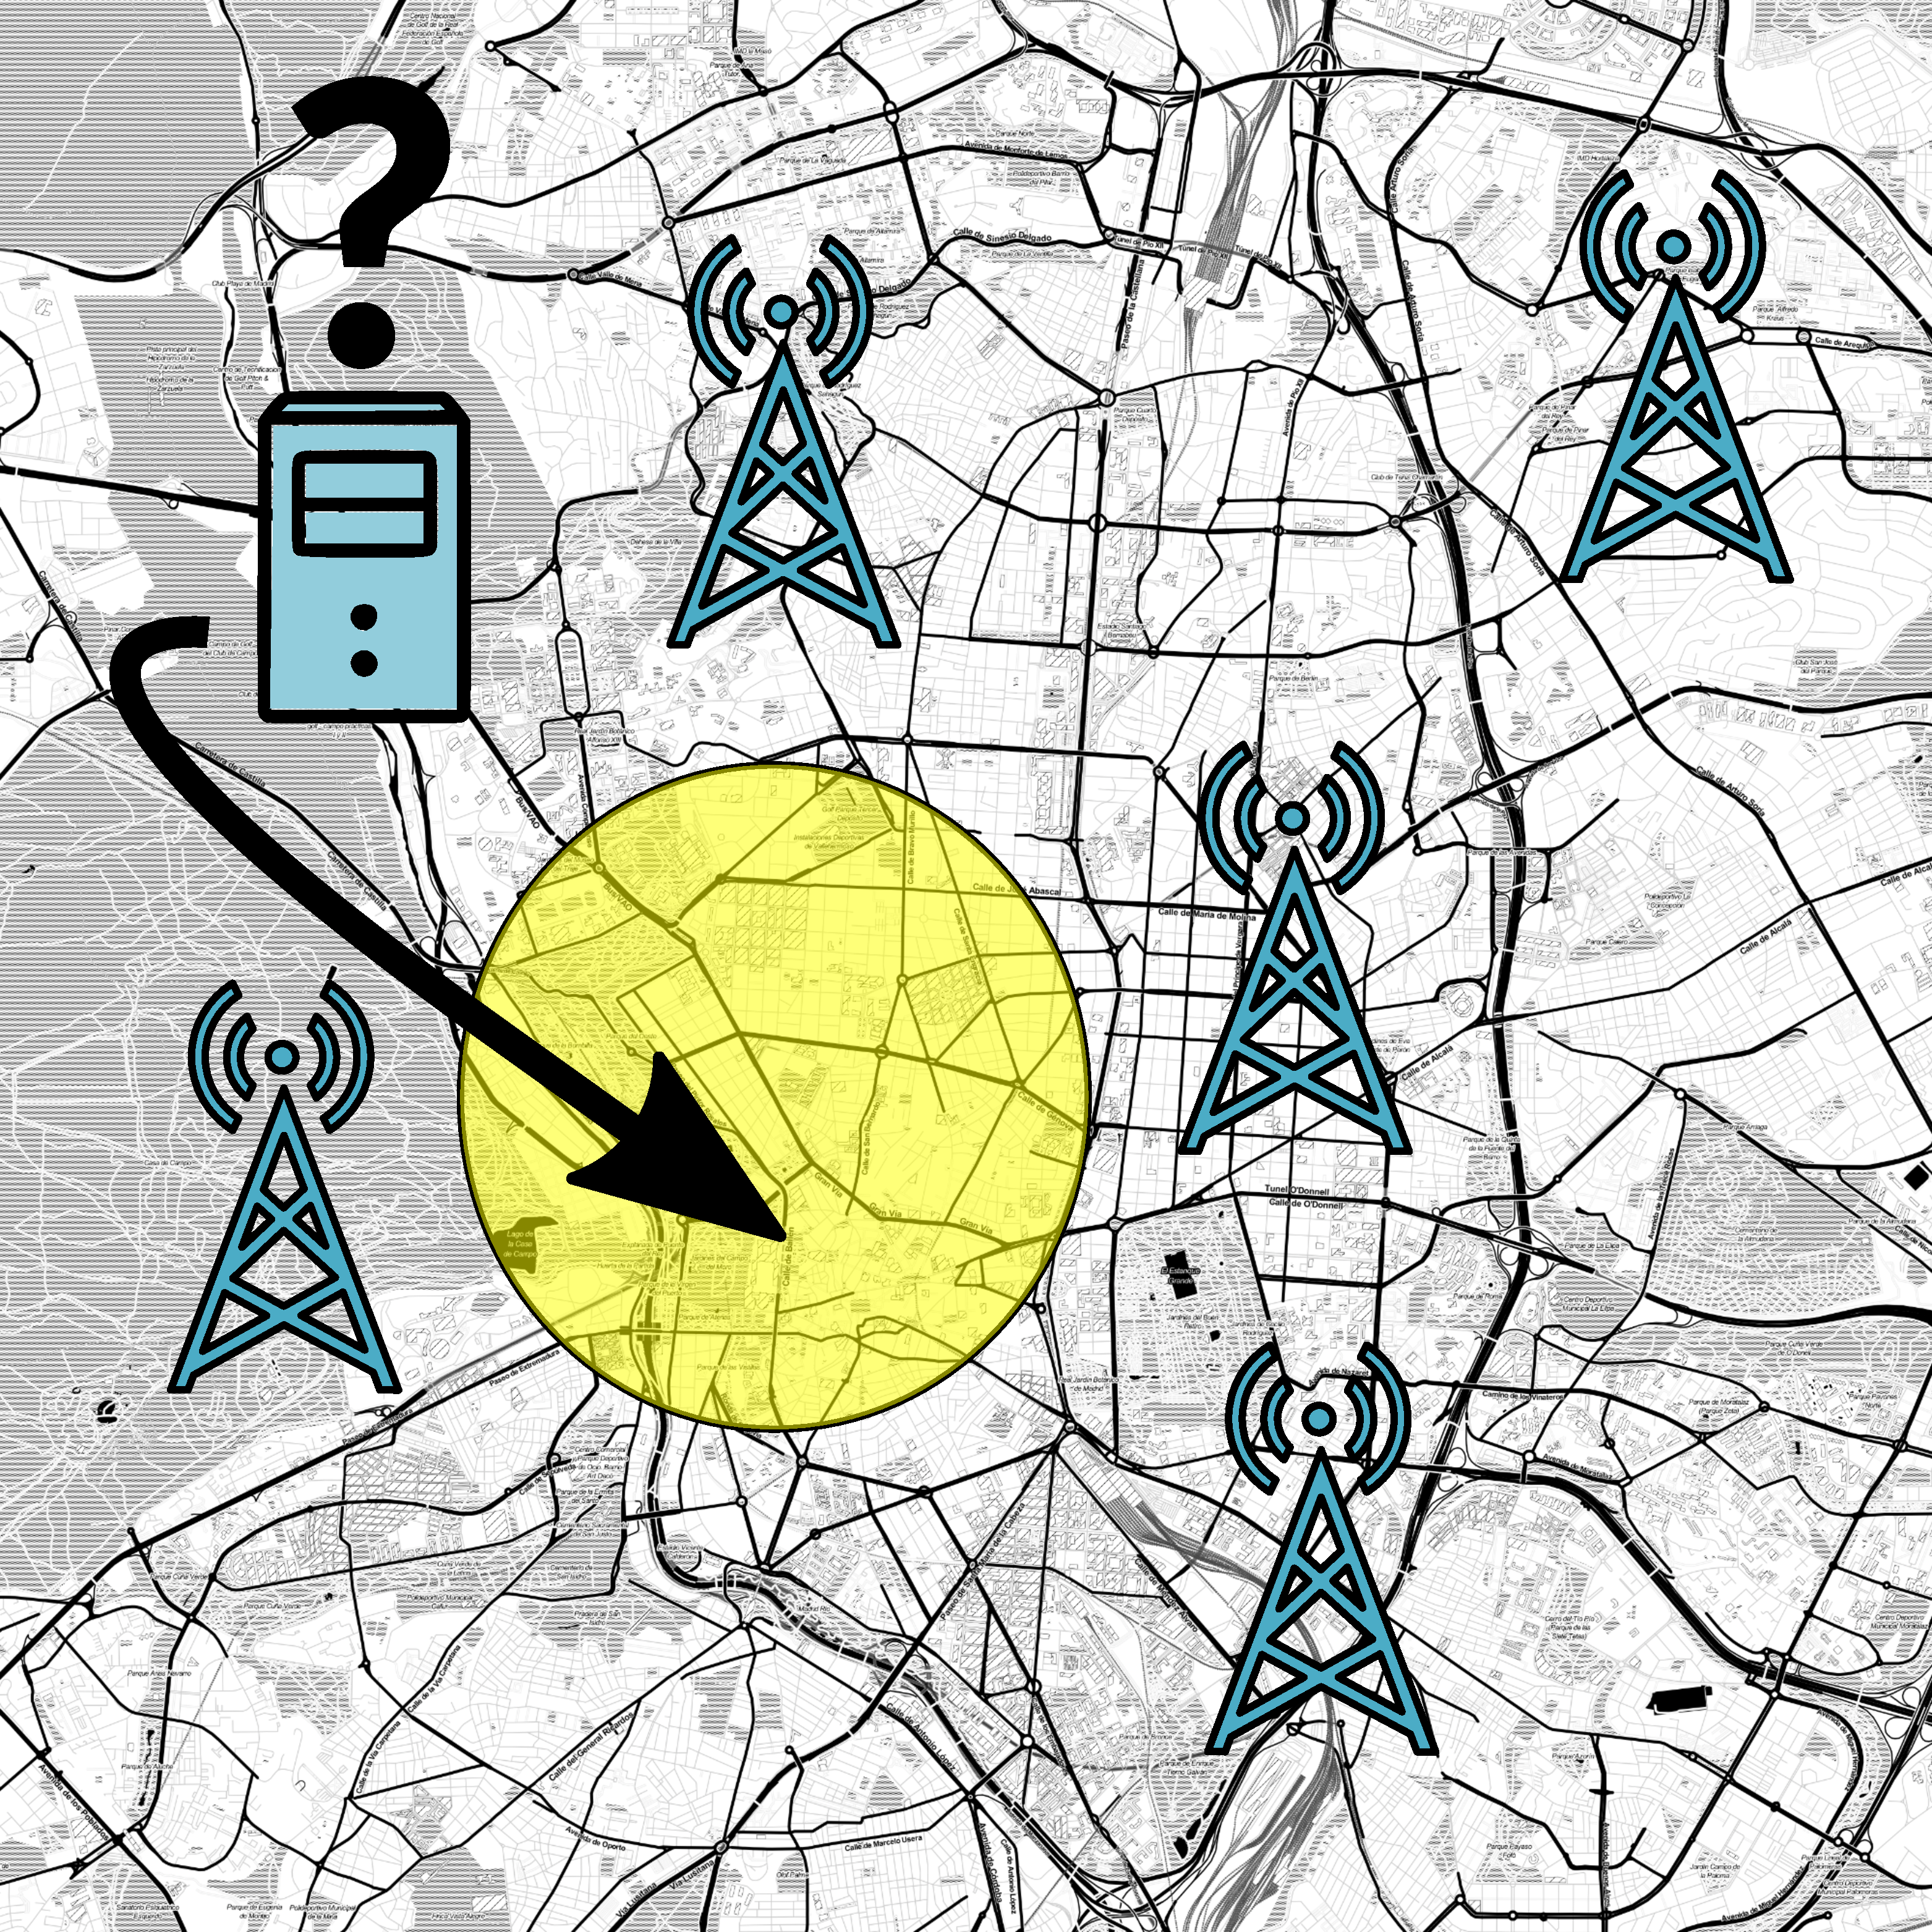
\includegraphics[width=.9\textwidth]{img/where-pop.pdf}}
            \caption{Location of BSs}
            \label{fig:bs-location}
        \end{figure}
    \end{minipage}
\end{frame}





\begin{frame}
    \frametitle{\secname}
    \framesubtitle{\subsecname}

    \begin{figure}
        \centering
        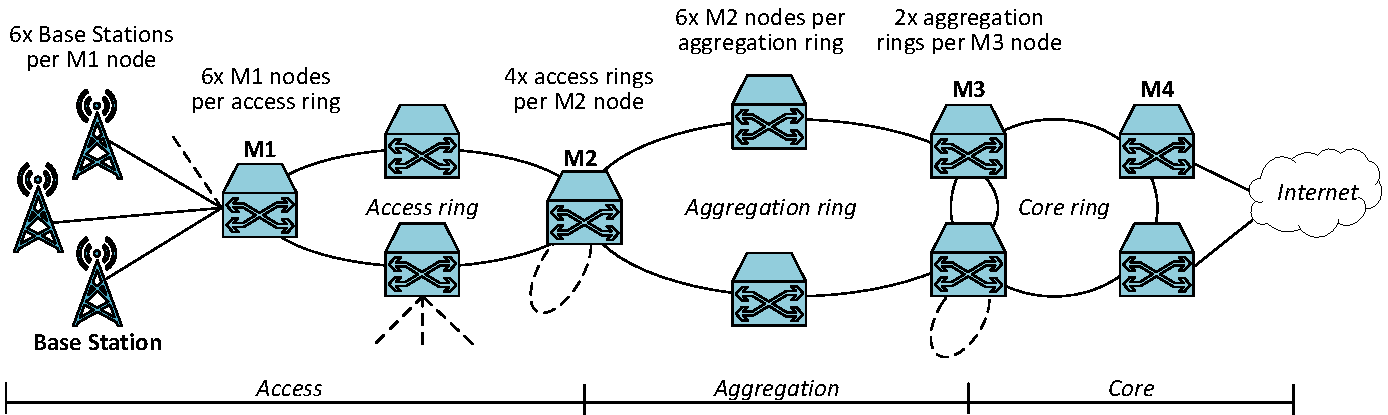
\includegraphics[width=1.0\textwidth]{img/infrastructure.pdf}
        \caption{Reference network infrastructure as illustrated\footnote{Author: Dr. Luca Cominardi.} in~\cite{8436847} and based on~\cite{itu.t.ref.arch}. }
        \label{fig:infrastructure}
    \end{figure}
\end{frame}





\begin{frame}
    \frametitle{\secname}
    \framesubtitle{\subsecname}

    Derive MEC PoP location considering:


    \begin{equation}
        \only<1>{RTT = \highlight{2d\cdot5\frac{\mu s}{km}}{fiber propagation} + 2M\cdot 50\mu s + UL + DL}
        \only<2>{RTT = 2d\cdot5\frac{\mu s}{km} + \highlight{2M\cdot 50\mu s}{ring propagation} + UL + DL}
        \only<3>{RTT = 2d\cdot5\frac{\mu s}{km} + 2M\cdot 50\mu s + \highlight{UL + DL}{radio propagation}}
        \label{eq:rtt-bad}
    \end{equation}

    \vfill

    \begin{itemize}
        \item $d$: distance between BS and MEC PoP
        \item $M$: network ring
        \item $UL$: Uplink propagation latency
        \item $DL$: Downlink propagation latency
    \end{itemize}

\end{frame}





\begin{frame}
    \frametitle{\secname}
    \framesubtitle{\subsecname}

    \centering{
        \only<1>{$m_M$: maximum distance between MEC PoP at ring $M$ and BS}
        \only<2>{$m_2$: maximum distance between MEC PoP at ring $2$ and BS}
    }
    \begin{figure}
        \centering
        \only<1>{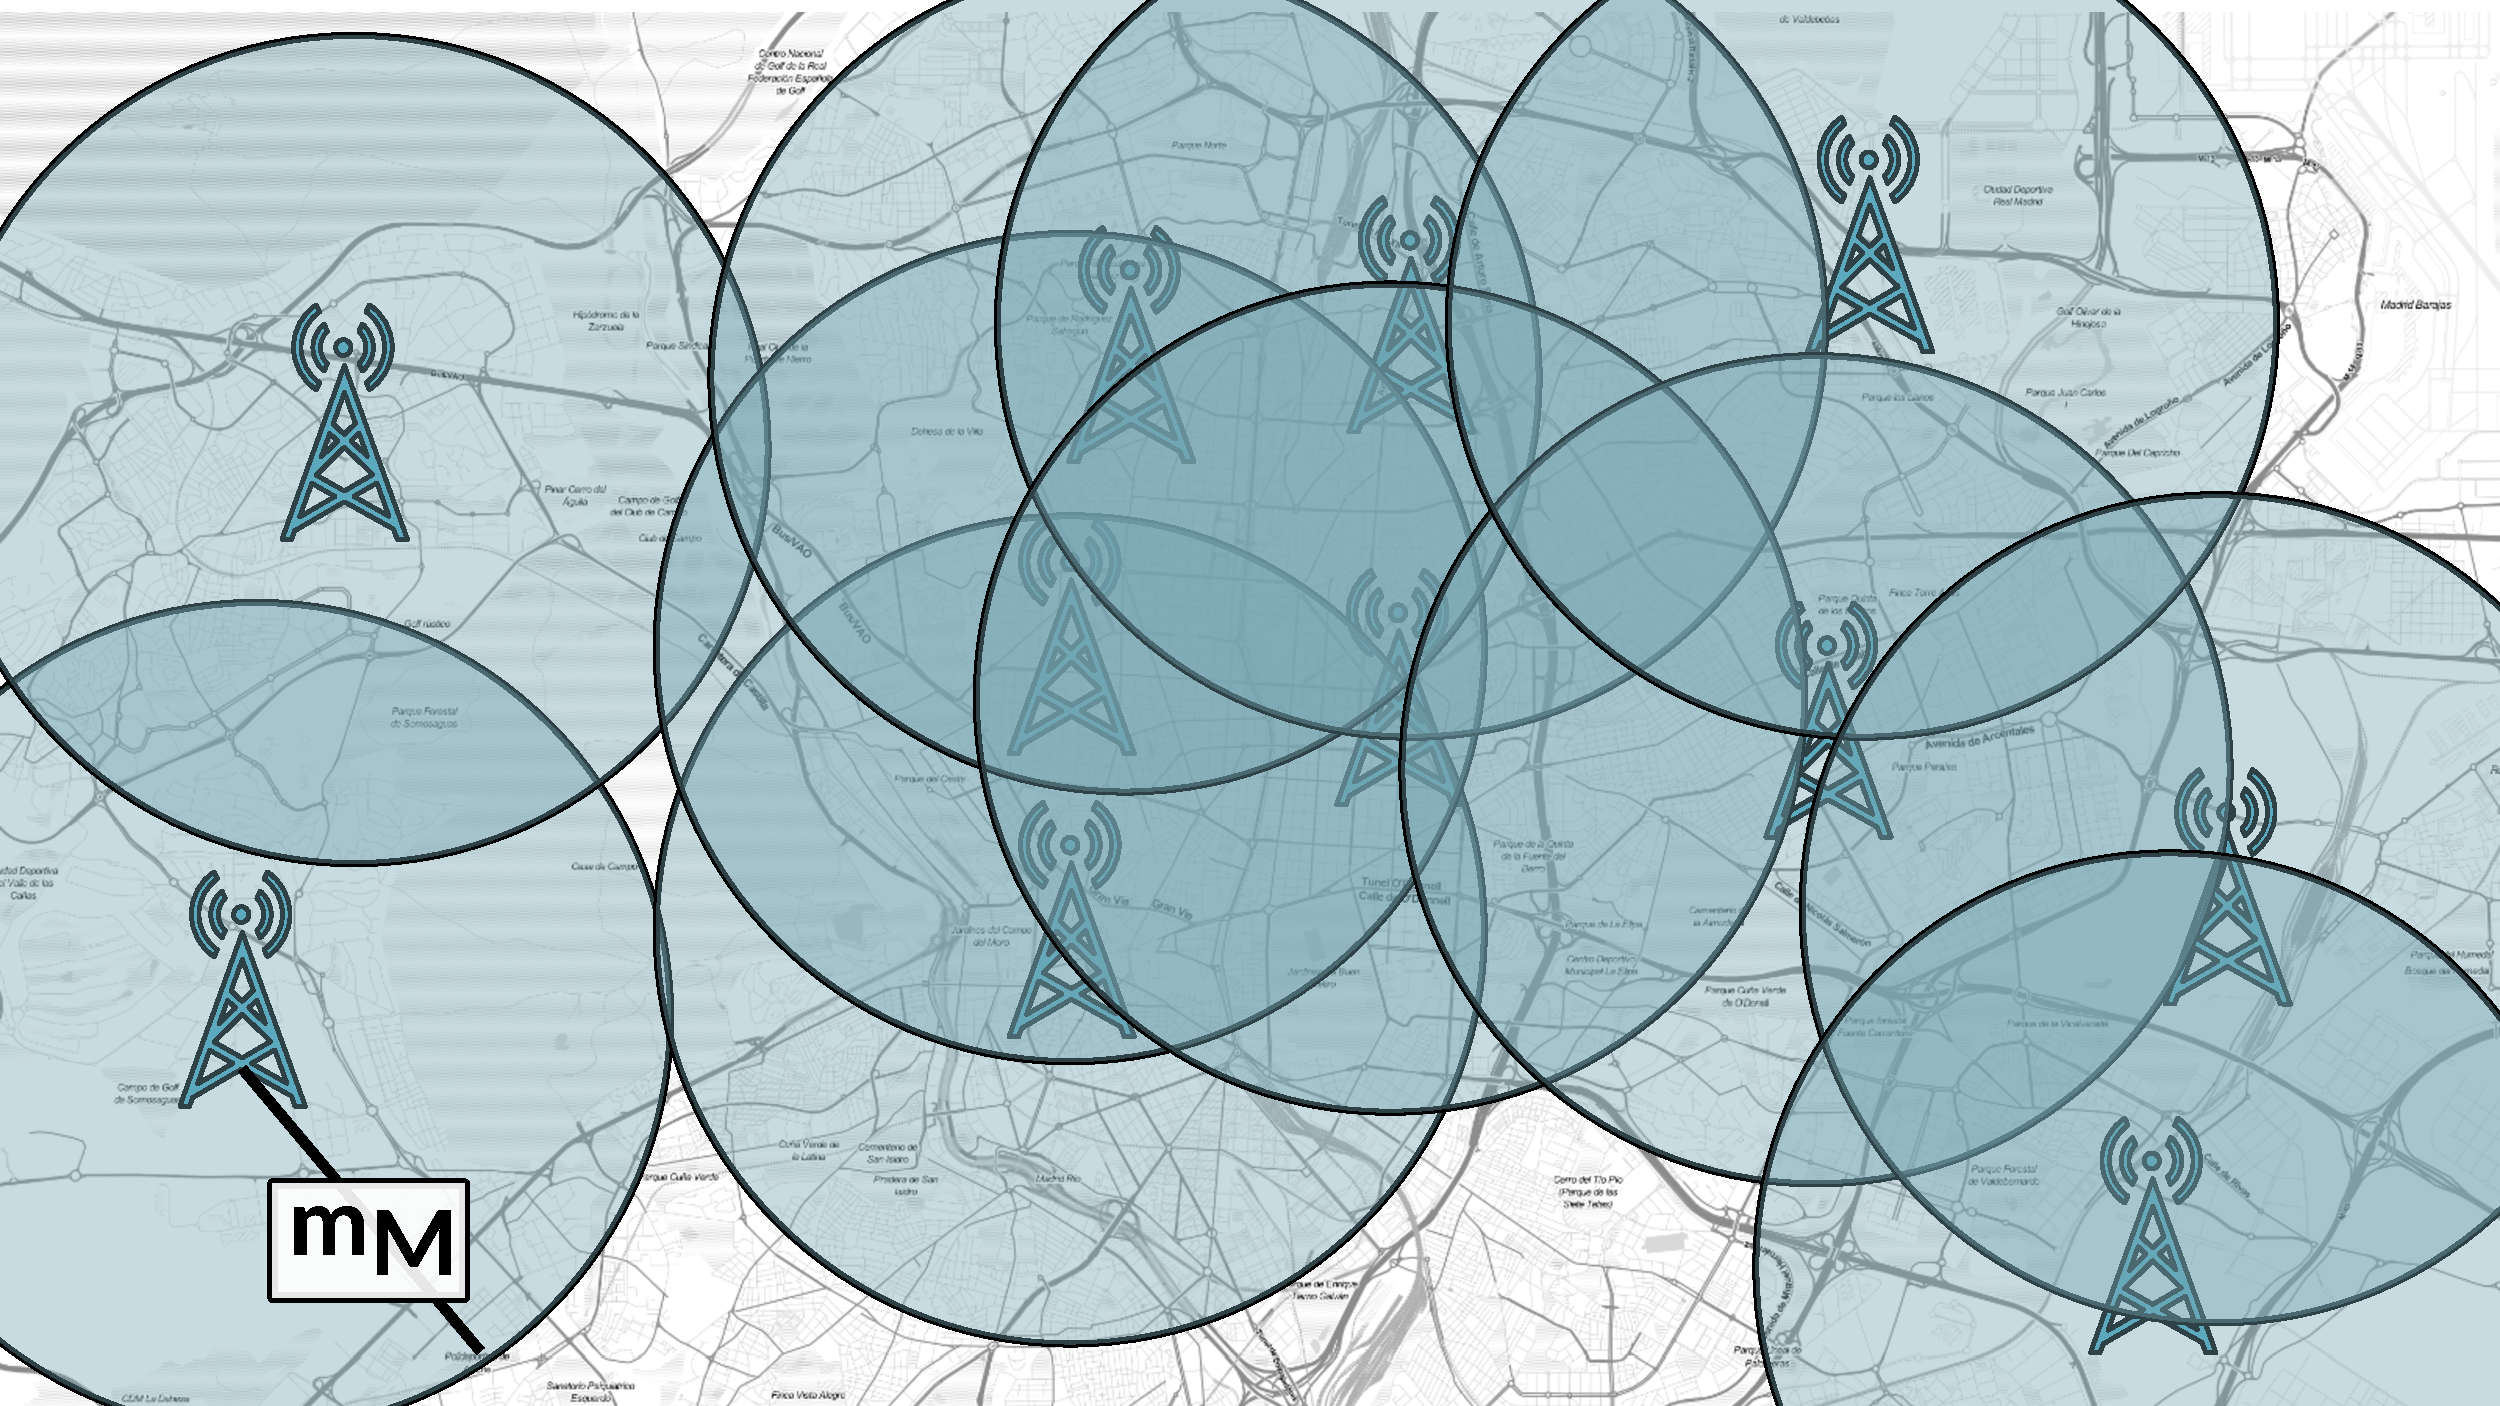
\includegraphics[width=0.7\textwidth]{img/generation-algo-1.pdf}}
        \only<2>{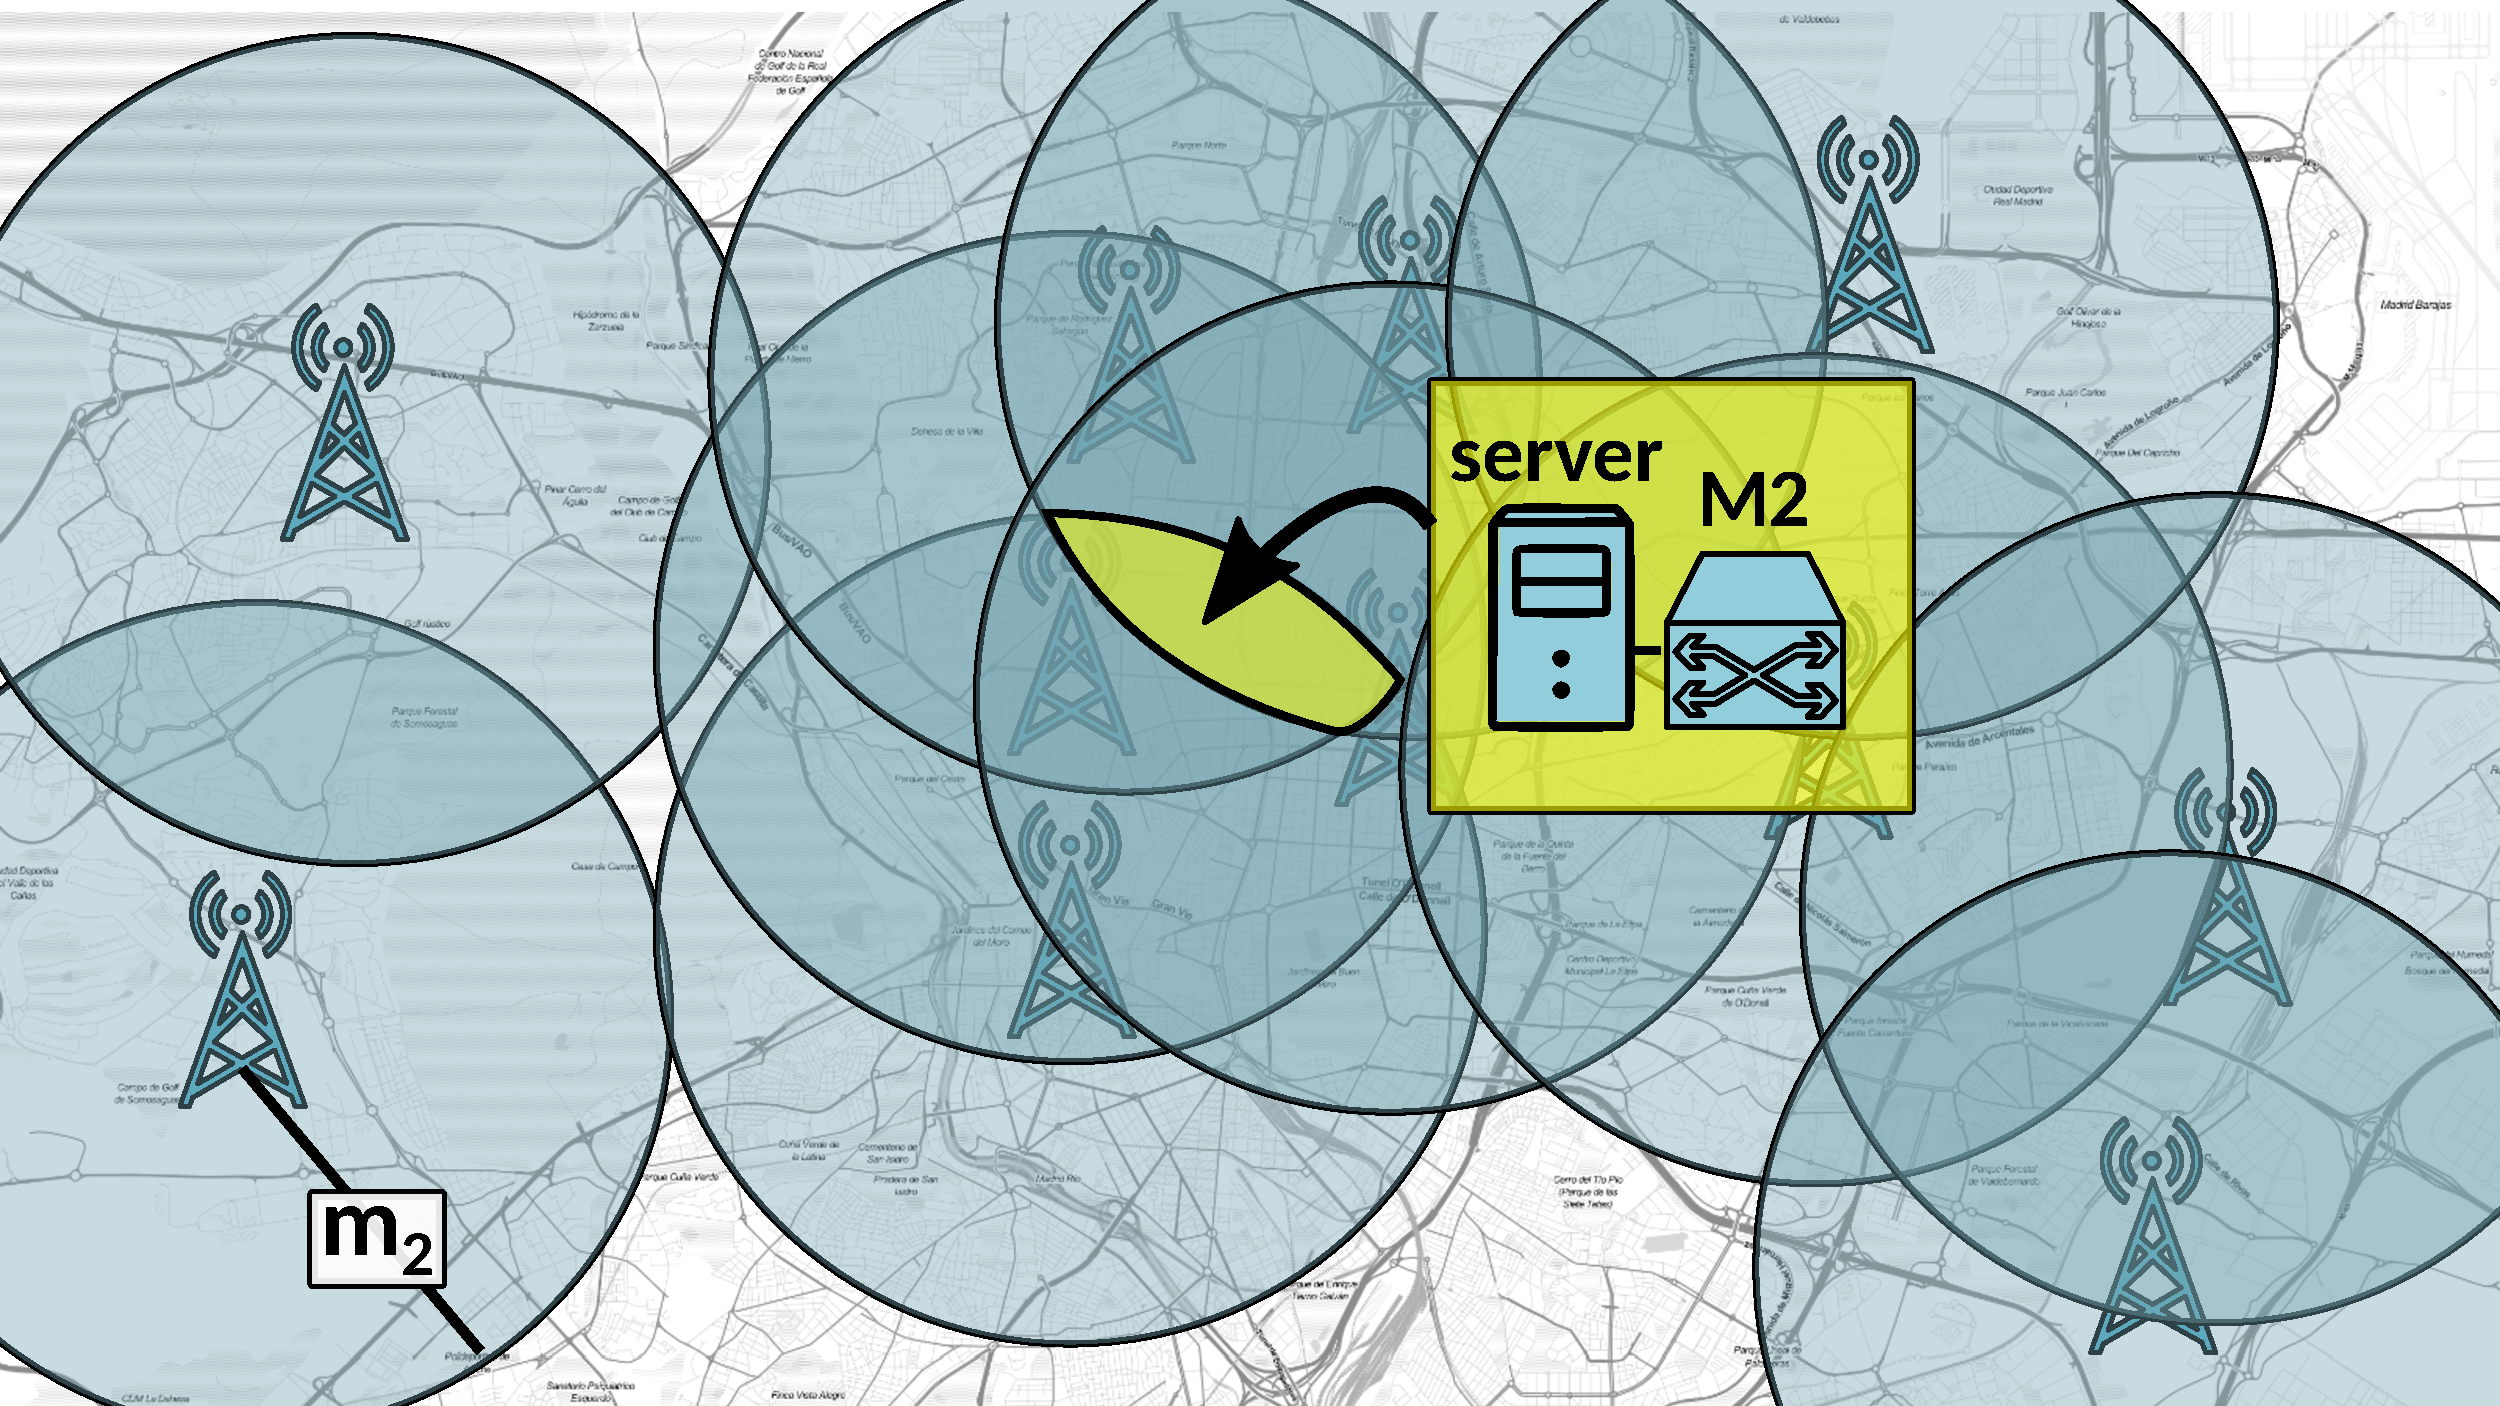
\includegraphics[width=0.7\textwidth]{img/generation-algo-2.pdf}}
        \caption{How to select MEC PoP location}
        \label{fig:algo-pop-location}
    \end{figure}
\end{frame}






\begin{frame}
    \frametitle{\secname}
    \framesubtitle{\subsecname}


\begin{figure}
    \centering
    % \comment{!!! @Jorge: this is still here!!! We need to improve the figures captions. It's hard to understand what the figures show only by looking at the pictures. It is not explained in the what $C_{A,M2}$ means. !!!}
    \subfigure[FDD 120 kHz 7s]{ 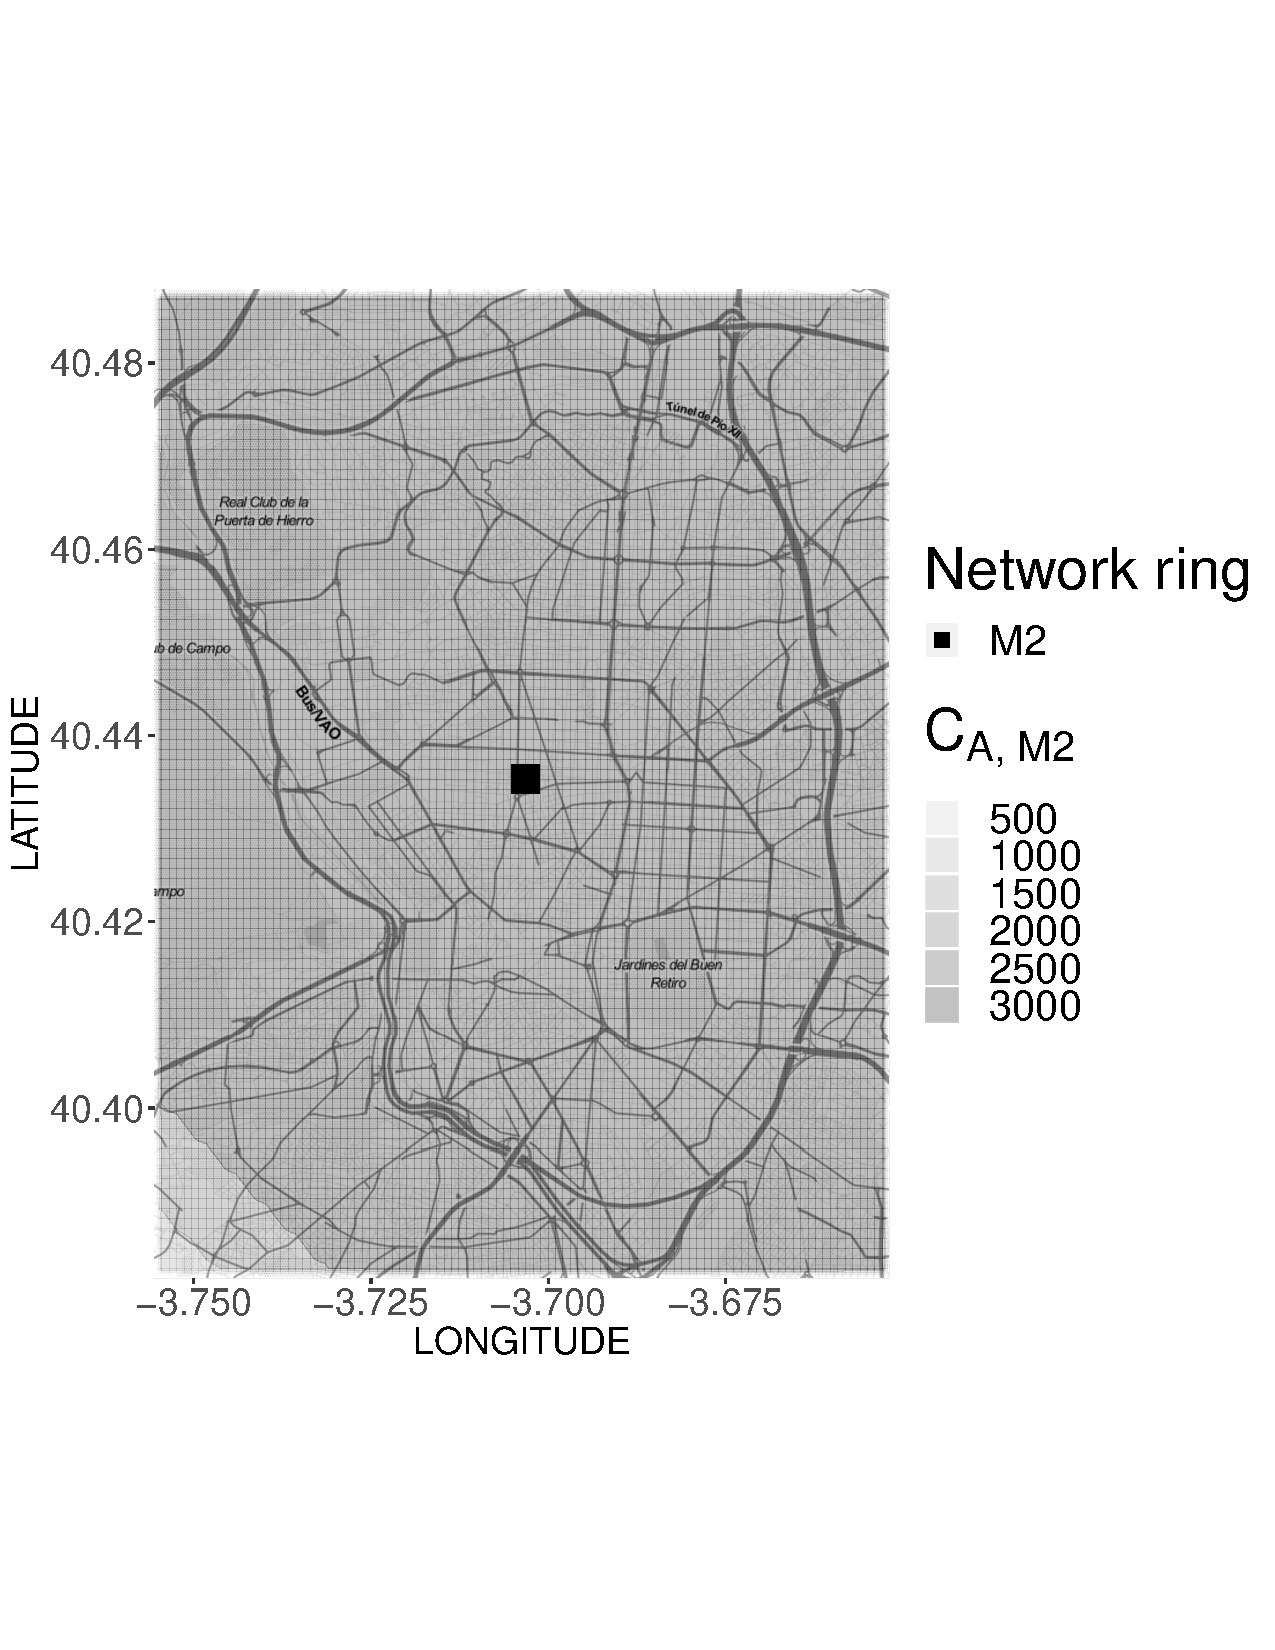
\includegraphics[clip, trim=0cm 2.7cm 0.25cm 3cm, width=0.35\textwidth]{img/madrid-ii-m2}}
        ~
    \subfigure[TDD 120 kHz 7s]{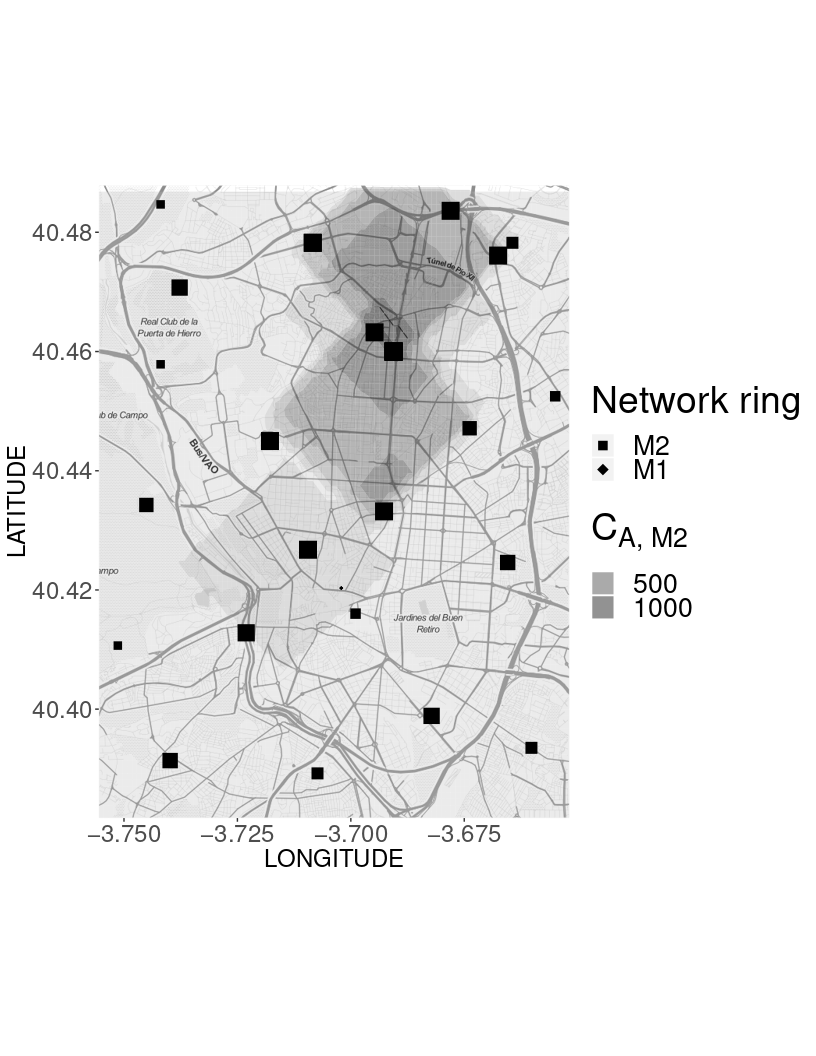
\includegraphics[clip, trim=0cm 2.7cm 0.25cm 3cm, width=0.35\textwidth]{img/madrid-i-iii-m2}}\\
    \caption{\textbf{Urban scenario} (Madrid city center) -- $C_{A,M2}=$covered BSs}
    \label{fig:madrid}
\end{figure}

\end{frame}





\begin{frame}

    \frametitle{\secname}
    \framesubtitle{\subsecname}

\begin{figure}
    \centering
    \subfigure[FDD 120 kHz 7s]{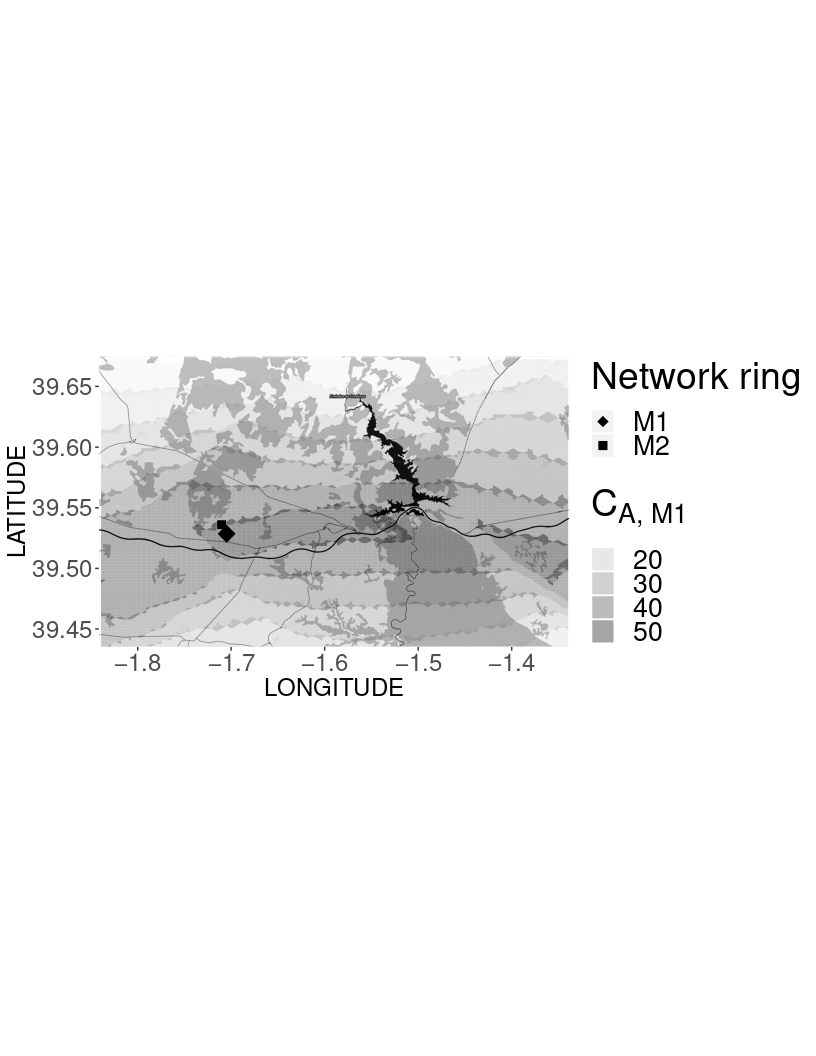
\includegraphics[clip, trim=0cm 8.5cm 0.25cm 6.7cm, width=0.45\textwidth]{img/hoces-del-cabriel-ii-m1}}
     ~                       
    \subfigure[TDD 120 kHz 7s]{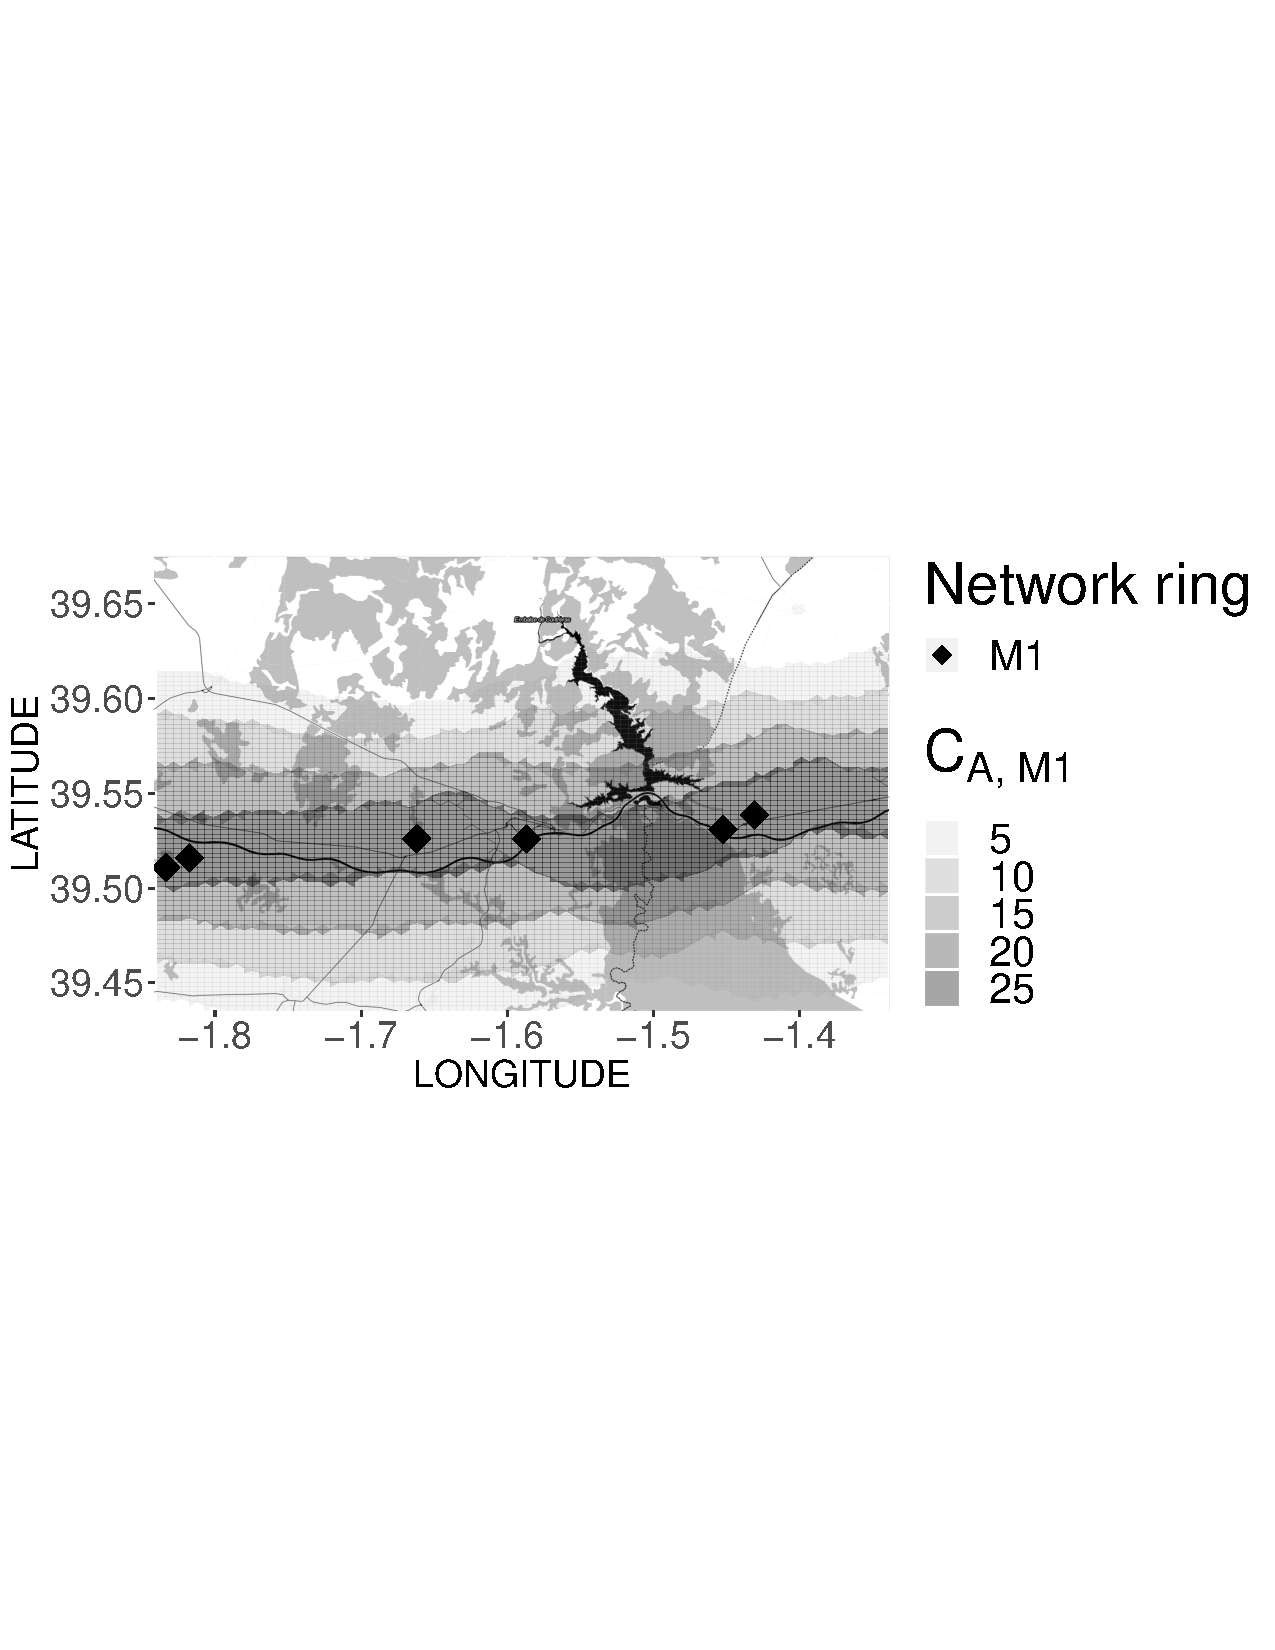
\includegraphics[clip, trim=0cm 8.5cm 0.25cm 6.7cm, width=0.45\textwidth]{img/hoces-del-cabriel-i-iii-m1}}\\
    \caption{\textbf{Highway scenario} (Hoces del Cabriel A3) -- $C_{A,M1}=$covered BSs by M1 MEC PoP}
    \label{fig:madrid}
\end{figure}

\end{frame}





\begin{frame}

    \frametitle{\secname}
    \framesubtitle{\subsecname}

    \begin{figure}[t]
        \centering
        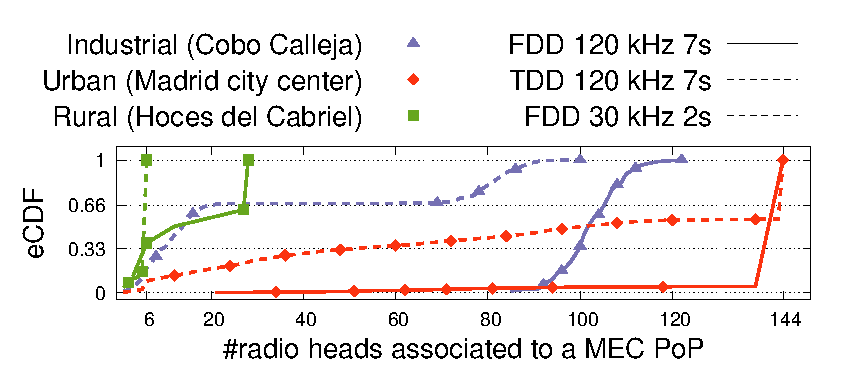
\includegraphics[width=.8\columnwidth]{img/cdfs}
        \vspace{1em}
        \caption{eCDF of the number of BSs assigned to a MEC PoP in the studied scenarios.}
        % \comment{LC: Increase the axis and label font size}
        \label{fig:cdfs}
    \end{figure}
\end{frame}


\subsection{Output}
\begin{frame}
    \frametitle{Outline}
    \tableofcontents[subsectionstyle=show/shaded/hide,sectionstyle=show/shaded]
\end{frame}

\begin{frame}
    \frametitle{Outline}
    Publications
    \begin{itemize}
        \item \fullcite{modelling-bs}
        \item \fullcite{5gen}
    \end{itemize}
    Open-source
    \begin{itemize}
        \item \url{github.com/MartinPJorge/mec-generator}
        \item \href{https://github.com/MartinPJorge/mec-generator/tree/5g-infra-gen}{5GEN R package}
    \end{itemize}
    

\end{frame}





\begin{frame}
    \frametitle{\insertsection}
    \textbf{Vertical services} (VS) contain:
    \begin{itemize}
        \item Virtual Network Functions (\textbf{VNFs}); and
        \item Virtual Links (\textbf{VLs}).
    \end{itemize}
\end{frame}


\section{NFV Orchestration in federated environments}
\subsection{State of the art}
\begin{frame}
    \frametitle{\insertsection}
    \textbf{Vertical services} (VS) contain:
    \begin{itemize}
        \item Virtual Network Functions (\textbf{VNFs}); and
        \item Virtual Links (\textbf{VLs}).
    \end{itemize}
\end{frame}



\section{NFV orchestration for 5G networks}
\begin{frame}
    \frametitle{\insertsection}
    \textbf{Vertical services} (VS) contain:
    \begin{itemize}
        \item Virtual Network Functions (\textbf{VNFs}); and
        \item Virtual Links (\textbf{VLs}).
    \end{itemize}
\end{frame}

\section{Scaling of V2N services: a study case}
\begin{frame}
    \frametitle{\insertsection}
    \textbf{Vertical services} (VS) contain:
    \begin{itemize}
        \item Virtual Network Functions (\textbf{VNFs}); and
        \item Virtual Links (\textbf{VLs}).
    \end{itemize}
\end{frame}

\section{Future work}
\begin{frame}
    \frametitle{\insertsection}
    \begin{itemize}
        \item integrate OKpi with RoS\footnote{robotic operating system}
        \item migration of robot remote driving component with OKpi
    \end{itemize}
\end{frame}


\begin{frame}
    \frametitle{Thanks}

    {\centering \huge
        Thanks for your attention!
    }
    \vfill
    OKpi is open-source, and it is implemented in python's placement module as FPTASMapper:
    \center{\url{https://github.com/MartinPJorge/placement}}
\end{frame}






\begin{frame}[allowframebreaks]
        \frametitle{References}
        % \bibliographystyle{amsalpha}
        % \bibliography{bibliography.bib}
        \printbibliography[heading=none]
\end{frame}







\section*{Details}
\begin{frame}
    \frametitle{\secname}
    \framesubtitle{Inhomogeneous Mattérn~II process}
    \begin{lemma}
    Given an \emph{inhomogeneous} marked PPP $X$ with \emph{intensity function} $\lambda$, the \emph{thinning} function $I_2$, and marks $m \sim \frac{1}{\lambda(x)}$, the resulting thinned point process, called \emph{inhomogeneous Mat\'ern~II}~PP, has the following average \emph{number of points} at $C$:
        \begin{equation}
            \mathbb{E}\left[ N(C) \right] := \int_C e^{-\int_{B(x,r)} \mathds{1}\left(\lambda(u) > \lambda(x) \right) \lambda(u) du} \lambda(x)\ dx
            \label{eq:inh-matern2-avg}
        \end{equation}
        where $r$ is the \emph{thinning} radius of $I_2$.
        \label{prop:inh-matern2-avg}
    \end{lemma}



    \vfill
    with
    \begin{equation}
        I_2(x,m, X, M_X) := \begin{cases*}
            1 & if $m = \min_{m' \in M_X}\big\{ (x',m'): x'\in B(x,r) \big\}$\\
            0 & otherwise
        \end{cases*}
        \label{eq:matern2}
    \end{equation}

\end{frame}





\begin{frame}
    \frametitle{\secname}
    \framesubtitle{Maximum distance between PoP and BS}


    The RTT considered is computed as
    \begin{equation}
        RTT := 2 l\left(\lVert x - m \rVert_1 \right) + 2 p(M) + UL + DL
        \label{eq:rtt}
    \end{equation}


    We find $m_M$, the maximum distance from MEC PoP $m$ to the BS at position $x$, as:
    \begin{equation}
        \lVert x-m \rVert_1 \le l^{-1}\left( \frac{RTT - 2p(M) - t_r}{2} \right)  = m_M
        \label{eq:max-dis}
    \end{equation}
    with $\lVert \cdot \rVert_1$ denoting the Manhattan distance.
\end{frame}




\end{document}
